\begin{frame}[allowframebreaks]{Destiny of Diffusions is decided early on}



\begin{itemize}
    \item As an example in the image domain consider  the availability of a rendering engine that takes as an input a computer program describing a scene (coordinates of objects, textures, light sources, auxiliary labels, etc ...). $V=\text{rendering}(X)$.\\
    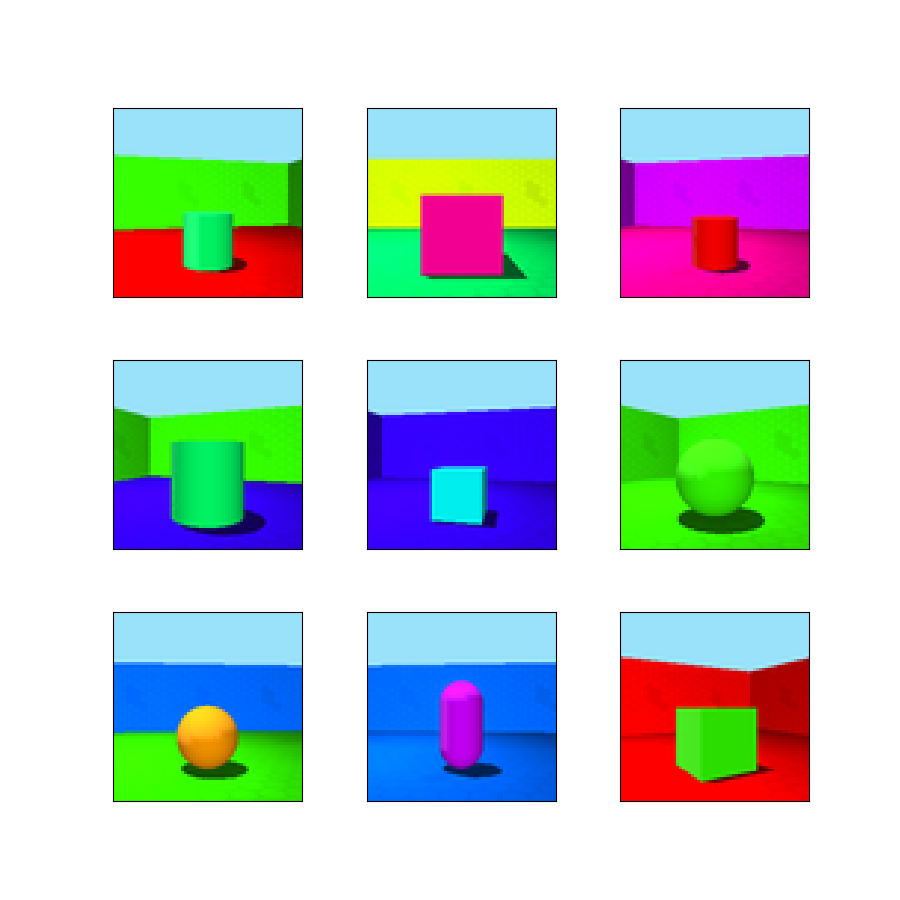
\includegraphics[scale=0.2]{figures/shapes3d-2.0.0.png}
\framebreak

\item Consider generative dynamics
    \begin{figure}[htbp]
    \centering
    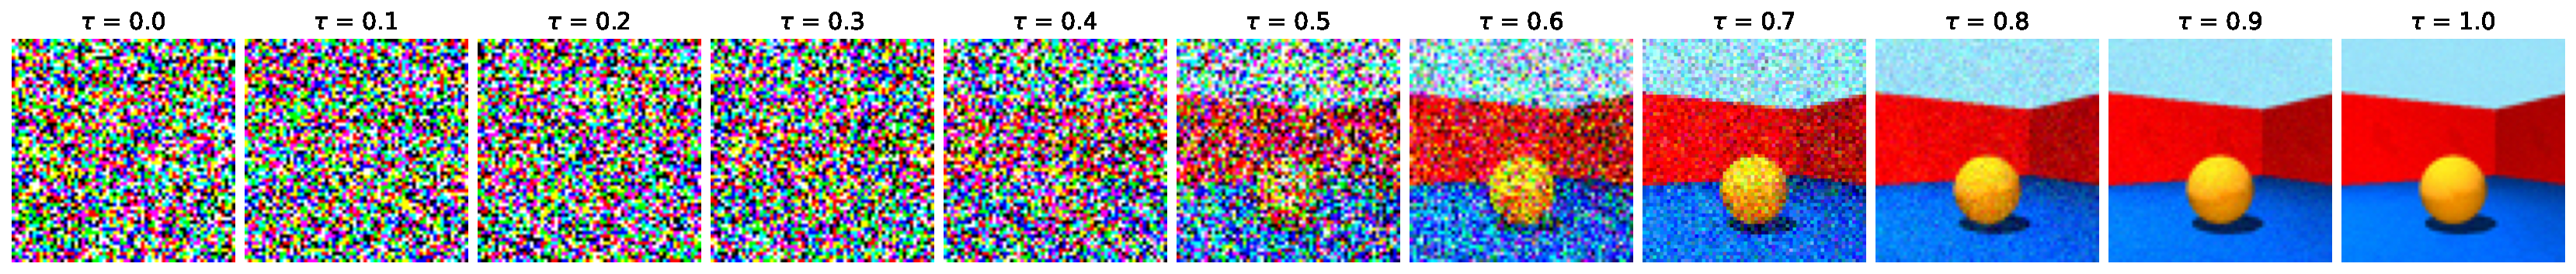
\includegraphics[width=\linewidth]{figures/noisy_balls.pdf}
    \caption{Evolution of generative dynamics vs $\tau$.}
    \label{fig:noise}
\end{figure}
\end{itemize}

\framebreak

Design of \textbf{forking} experiments:

\begin{figure}[htbp]
    \centering
    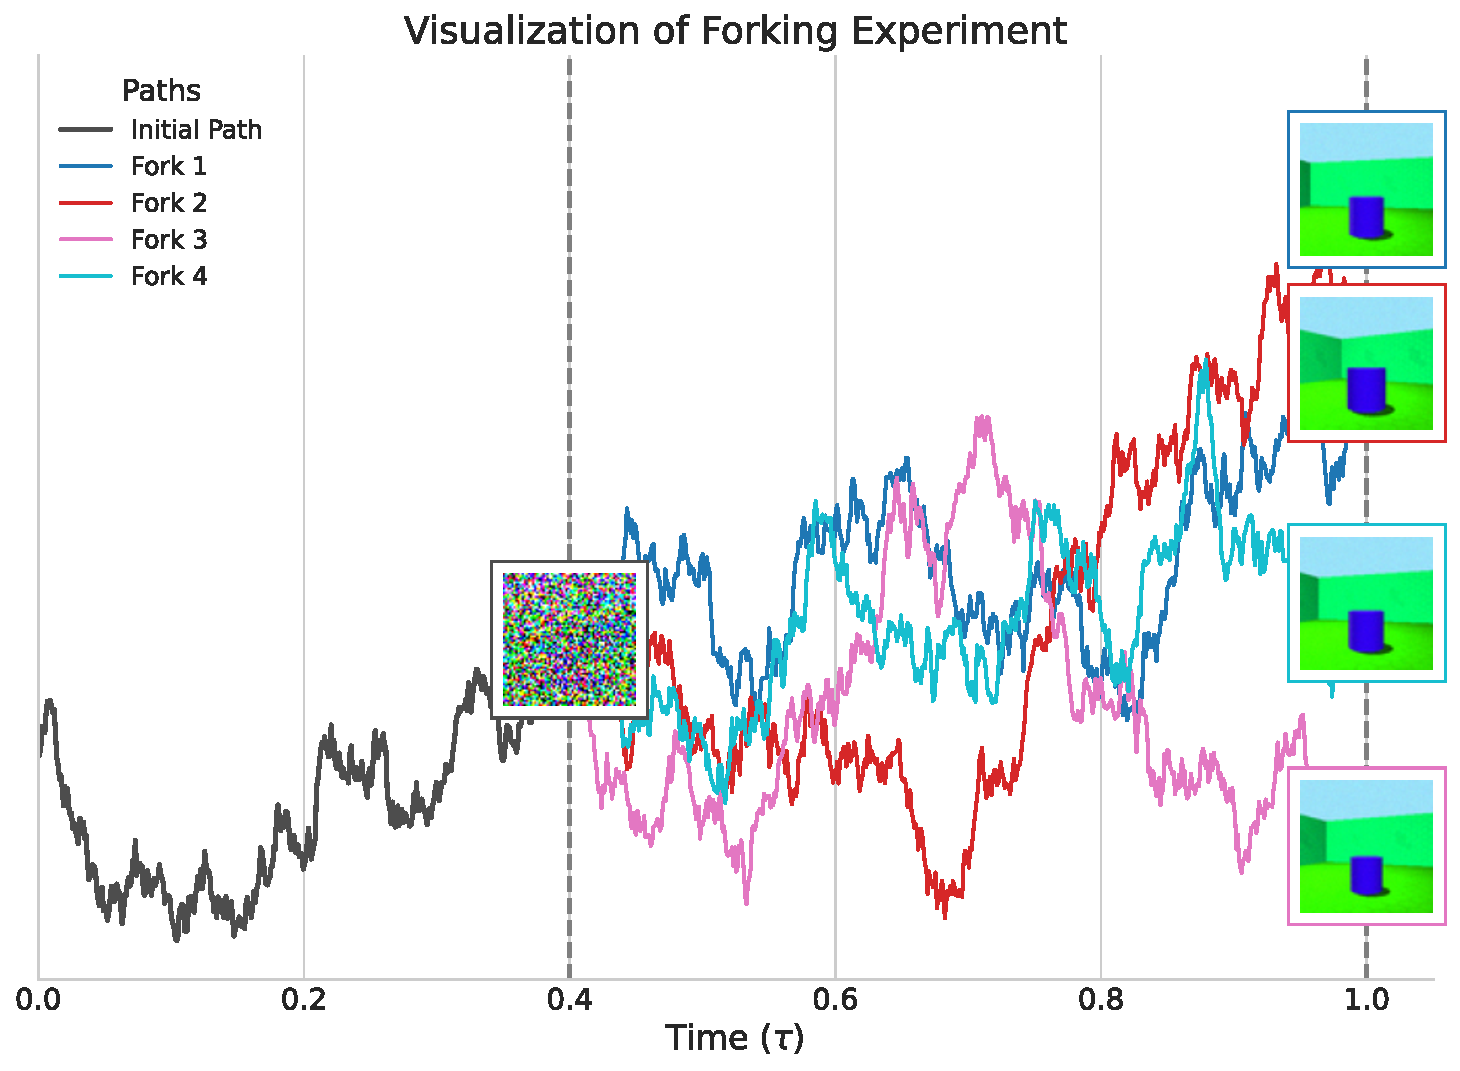
\includegraphics[width=0.6\linewidth]{figures/forking_visualization.pdf}
    \caption{  The image at time $\tau = 0.4$ is quite noisy. In the final generations after forking, the images exhibit coherence in the labels \textit{shape}, \textit{wall hue}, \textit{floor hue}, and \textit{object hue}. However, there is variation in \textit{orientation} and \textit{scale}.}
    \label{fig:forking_visualization}
\end{figure}
\framebreak

This phenomenon holds true for much more complex datasets! Moreover, it has been observed that by (linearly) probing the neural activations you can predict the fate of the diffusion

\begin{figure}
    \centering
    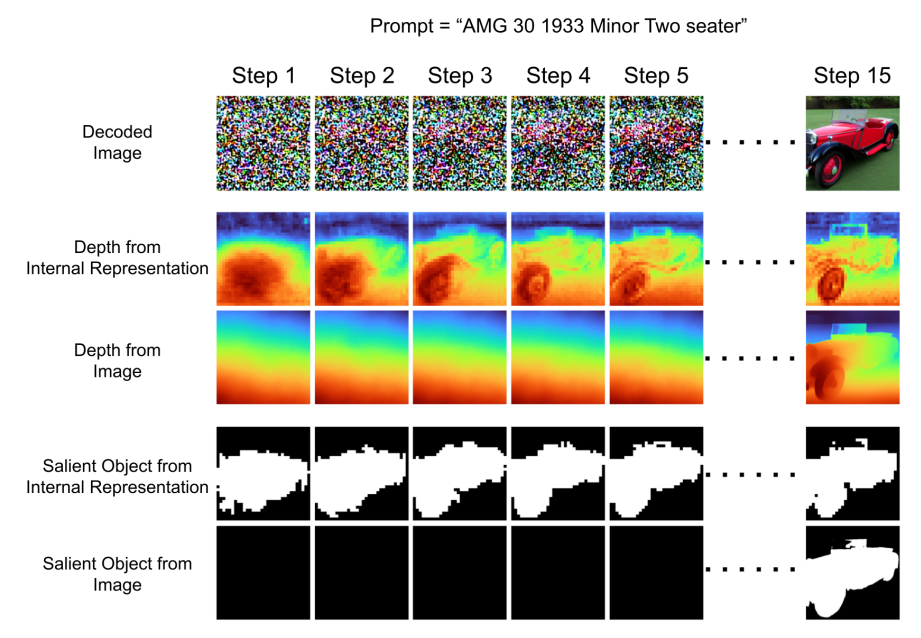
\includegraphics[width=0.7\linewidth]{figures/segm_map.PNG}
   % \caption{Caption}
    \label{fig:enter-label}
\end{figure}



\end{frame}
\begin{frame}{Plan for the work}
\begin{itemize}
    \item Show that a class of generative models (which contains diffusion models) can be written as a system of \textbf{simulated} Nonlinear Filtering (NF) equations.
    \item (Slight) generalization of classical NF results to accommodate for arbitrary filtrations, non-zero initial conditions...
    \item Derive expressions for MI evolution between generative dynamics and latent abstractions.
\end{itemize}
    Mechanistic conjecture: use this formalization to design experiments to investigate inner workings of neural networks in diffusion models (and the generalised class).
\end{frame}

\begin{frame}[allowframebreaks]{Nonlinear Filtering}

\begin{itemize}
\item Consider two random variables $Y_t$ and $X$, corresponding to a stochastic\textbf{ measurement} process $Y_t$ of some underlying \textbf{latent abstraction} $X$ (a random variable $X:\Omega\rightarrow \cS$).
\item Consider natural filtration $\cF^{Y,X}_t=\sigma( Y_{0\leq s\leq t},X )$
\item Suppose on $(\Omega,\cF^{Y,X}_{T},\mathrm{P})$ the process $\{(Y_{0\leq t\leq T},X),\cF^{Y,X}_{0\leq t\leq T}\}$ has representation
\begin{equation}\label{eq:param_sde}
    Y_t=Y_0+\int_0^t H(Y_s,X,s) \dd s+ W_t,
\end{equation}
where $\{W_{0\leq t\leq T},\cF^{Y,X}_{0\leq t\leq T}\}$ is a Brownian motion and $H$
is an \textit{observation} process. 
% All (standard) technical assumptions considered in this work are available in \Cref{app:assumptions}.
\framebreak
  \begin{itemize}
    \item The nonlinear filtering problem asks: given access to observations $Y_t$ ( $\cF^Y_t=\sigma(Y_{0\leq s\leq t})$) , how can we estimate the posterior distribution of $X$ (or some function of $X$)?
    \[\pi^{\cF^Y}_t(A)=\PO[ X\in A\g {\cF_t^Y}]\]

    \item \textbf{The key idea is to rewrite Equation \ref{eq:param_sde} into an equivalent form that no longer explicitly depends on $X$.}
  \end{itemize}
\end{itemize}

\end{frame}

\begin{frame}[allowframebreaks]{Key ingredients (without proofs)}
\begin{itemize}
    \item Consider the family of growing filtrations $\ctF_t=\sigma(\ctF_0\cup \sigma(Y_{0\leq s\leq t}-Y_0))$, where $\sigma(Y_0)\subseteq \ctF_0\subseteq \sigma(X,Y_0)$
    \item $\ctF_0$: modulate between the two extreme cases of knowing only $Y_0$ to the case of complete knowledge of the whole $X$.
   % \item The conditional probability measure $\PO[ X\in A\g \mathcal{R}_t]$ is well defined and is equal to $\pi^\ctF_t(A)$.
    \item $Y_t$ is obviously adapted to any $\ctF_t$, but the representation $Y_t=Y_0+\int_0^t \underbrace{H(Y_s,X,s)}_{\text{this needs } X} \dd s+ W_t$ is (in general) not.
\end{itemize}
\framebreak

\begin{theorem}\label{innovation_theo}
The process $\{Y_{0\leq t\leq T},\ctF_{0\leq t\leq T}\}$ has \gls{SDE} representation 
\begin{equation}\label{genh_sde}
Y_t=Y_0+\int_0^t \E_{\PO}(H(Y_s,X,s)\g \ctF_s)\dd s + {W}^{\cR}_t,    
\end{equation}
where $\{{W}^{\cR}_{0\leq t\leq T},\ctF_{0\leq t\leq T}\}$ is a Brownian motion.
\end{theorem}

  \begin{itemize}
    \item The Theorem states that $Y_t$ has an\textbf{ equivalent representation} (Equation \ref{genh_sde}) adapted to a \textbf{smaller filtration}, rather than to both $Y_t$ and $X$.
    \item This \textbf{does not mean} $Y_t$ is \textbf{independent} of $X$, only that an observer unaware of $X$ can still construct a valid stochastic model for $Y_t$.
  \end{itemize}

\framebreak

\begin{theorem} \label{theo_girsa}
Define $\tilde{W}_t\defeq Y_t-Y_0$ and a new probability space $\cctU$ via the measure $\PT(A)=\E_{\PO}\left[ \mathbf{1}(A)({\psi^{\ctF}_T})^{-1}\right]$, for $A\in \ctF_T$, where 
\begin{equation}\label{radonniko}
\psi^{\ctF}_t\defeq \exp(\int_0^t \E_{\PO}[H(Y_s,X,s)\g\ctF_s]\dd Y_s-\frac{1}{2}\int_0^t\norm{\E_{\PO}[H(Y_s,X,s)\g\ctF_s]}^2 \dd s ),
\end{equation}
and  
$$\PT\g_{\ctF_t}=\E_{\PO}\left[ \mathbf{1}(A)\E_\PO[({\psi^{\ctF}_T})^{-1}\g\ctF_t]\right]=\E_{\PO}\left[ \mathbf{1}(A)({\psi^{\ctF}_t})^{-1}\right].$$ 


Then, the stochastic process $\{\tilde{W}_{0\leq t\leq T}, \ctF_{0\leq t\leq T}\}$ is a Brownian motion on the space $\cctU$. $\tilde{W}_t$ is independent of any $\ctF_0$ measurable random variable under the measure $\PT$. 
Moreover, it holds that for all $\mathcal{R}'_t\subseteq \mathcal{R}_t$, 
$\PT\g_{\mathcal{R}'_t}=\mathrm{Q}^{\mathcal{R}'}\g_{\mathcal{R}'_t}
$.

\end{theorem}
\framebreak
We can combine together the results and apply \textbf{Bayes'theorem}:
\begin{equation}
  \PO[ X\in A\g \mathcal{R}_t]=  \E_{\PO}\left[ \mathbf{1}(A)\g\ctF_t\right]=\frac{\E_{\PT}\left[ \frac{\dd \PO}{\dd \PT} \mathbf{1}(A)\g\ctF_t\right]}{\E_{\PT}\left[ \frac{\dd \PO}{\dd \PT}\g\ctF_t\right]}
\end{equation}

Remember: under $\PT$ now $\{Y_t-Y_0,\ctF_t\}$ is a Brownian motion! 
%In simple cases you know it in the following form
%\begin{equation*}
%  \int_A p(x\g r)\dd x = \int_A q(x\g r)\frac{p(x)}{q(x)}\dd x/(\int q(x\g r)\frac{p(x)}{q(x)}\dd x ) 
%\end{equation*}
\framebreak

The posterior probability can be obtained as the solution of an \gls{SDE} which is driven by $Y_t$
\begin{theorem} 
The measure-valued process $\pi^\ctF_t=\PO[ X\in A\g \mathcal{R}_t]$ solves in weak sense
    \begin{flalign}
        \pi^\ctF_t=\pi^\ctF_0+\int_0^t \pi^\ctF_s\left(H-\langle \pi^\ctF_s,H\rangle\right) \left(\dd Y_s-\langle \pi^\ctF_s,H\rangle\dd s\right)
    \end{flalign}
%where the initial condition $\pi_0$ satisfies $\pi^\ctF_0(A)=\PO[X\in A\g \ctF_0]$.
\end{theorem}
\begin{itemize}
    \item $\langle \pi^\ctF_t,H\rangle$ is what I expect $H$ to be, given my knowledge of $\ctF_t$, also written as $\E_{\PO}[H(X,Y_t,t)\g \ctF_t]$
    \item $\dd Y_t-\langle \pi^\ctF_t,H\rangle$ is the \textit{innovation process}
\end{itemize}
\framebreak
We conclude our excursion by quantifying the Mutual Information content across time.
For \textit{any} $\phi(X)$, with $\ctF_0=\sigma(\phi,Y_0)$:
\begin{theorem}
The mutual information $\cI(Y_{0\leq s\leq t};\gX)$  is equal to 
    \begin{equation}\label{MI_eq}
        \cI(Y_{0};\gX)+ \frac{1}{2}\E_{\PO}\left[ \int_0^t\norm{\E_{\PO}[H(X,Y_s,s)\g \cF^{Y}_s]-\E_{\PO}[H(X,Y_s,s)\g \ctF_s]}^2 \dd s \right].
    \end{equation}
  
\end{theorem}
\begin{itemize}
    \item Compare the best possible prediction of $H$ \textit{with or without} observation of $\phi(X)$. The larger the difference, the higher the Mutual Information.
\end{itemize} 
\framebreak
The mutual information between $\gX$ and the measurements depends on
\begin{itemize}
    \item   how much the amplitude of $H$ is impacted by knowledge of $\gX$ 
    \item the \textit{number} of elements of $H$ which are impacted (informally, how much localized vs global is the impact of $\gX$).
   \item This defines an \textit{hierarchy} of importance among latent factors.
\end{itemize}
\framebreak

The posterior $\pi_t$ is a \textbf{sufficient statistic} for any $\sigma(X)$ measurable random variable when starting from the measurement process. It is the maximal compression of $Y_{0\dots t}$ which has the same predictive power about $X$.

\begin{Theorem}\label{sufficient_statistic}
For any $\cF^Y_t$ measurable random variable $\tilde{Y}_t:\Omega\rightarrow \Psi$, the following inequality holds:
\begin{equation}\label{eq:dpi}
    \cI(\tilde{Y};\gX)\leq \cI(Y_{0\leq s\leq t};\gX).
\end{equation}

For a given $t\geq 0$, the measurement process $Y_{0\leq s\leq t}$ and $X$ are \textit{conditionally}-independent given $\pi_t$. This implies that $\PO(A\g \sigma(\pi_t))=\PO(A\g \cF^Y_t),\quad \forall A\in\sigma(X)$. Then
$\cI(Y_{0\leq s\leq t};\gX)=\cI(\pi_t;\gX)$ (i.e. \ref{eq:dpi} is attained with equality).
\end{Theorem}






\end{frame}


\begin{frame}[allowframebreaks]{Generative modelling}


\begin{itemize}
    \item We are interested in \textbf{generative models} for a given $\sigma(X)$-measurable random variable $\rX$
{\color{red}
    \item A generative model can be built simulating any stochastic process $Y_t$ satisfies $Y_T=\rX,\quad \PO-a.s.$ (Assumption 1).}
    \item Strategy: starts from a process with $\cF^{Y,X}$ adapted representation which you know satisfies Assumption 1
    \item Using the change of filtration tricks simulate the $\cF^{Y}$ adapted system 
    \begin{equation}\label{eq:system}
\begin{cases}
\pi_t=\pi_0+\int_0^t \pi_s\left(H-\langle \piphis,H\rangle\right) \left(\dd Y_s-\langle \piphis,H\rangle\dd s\right),\\
Y_t=Y_0+\int_0^t \langle \piphis,H\rangle \dd s+{W}^{\cF^Y}_t,    
\end{cases}
\end{equation}
\item As an example, Diffusion models can be written as a \textbf{particular case} of the original equations ($H(Y_t,X,t)=\frac{1}{2}Y_t -\frac{\exp(-\frac{(T-t)}{2})V-Y_t}{1-\exp(-(T-t))}$).
%\item Select the function $H$ as
%   \begin{equation}
%       H(Y_t,X,t)=\frac{1}{2}Y_t -\frac{\exp(-\frac{(T-t)}{2})V-Y_t}{1-\exp(-(T-t))}
 %  \end{equation}
%\item $\E[H(Y_t,X,t) \g \cF^Y_t]=\frac{1}{2}Y_t -\frac{\exp(-\frac{(T-t)}{2})\E[V \g \sigma(Y_t)]-Y_t}{1-\exp(-(T-t))}$
%\item The generative dynamics have then form $\dd Y_t=\frac{1}{2}Y_t -\frac{\exp(-\frac{(T-t)}{2})\E[V \g \sigma(Y_t)]-Y_t}{1-\exp(-(T-t))}+\dd W^{\cF^Y}_t$ (cfr with beginning of presentation!)
%\item Those dynamics can be interpreted as \textbf{implicit} simulation of the system eq.\ref{eq:system}
\end{itemize}


\framebreak
\begin{figure}
\scalebox{0.7}{
\begin{tikzpicture}[>=stealth, node distance=2cm]

% Define the nodes
\node(X){\color{blue}$X$};
\node[below= 1cm of X] (Y0) {\color{darkgreen}$Y_0$};
\node[right of= Y0] (Y1) {\color{darkgreen}$Y_1$};
\node[right of= Y1] (Y2) {\color{blue}$Y_2$};
\node[right of= Y2] (Y3) {\color{blue}$Y_3$};


% Arrows from X to Y
\draw[->] (X) -- (Y0);
\draw[->] (X) -- (Y1);
\draw[->] (X) -- (Y2);
\draw[->,color=blue] (X) -- (Y3);

% Pi nodes and arrows
\node[below =1cm of Y0] (pi0) {\color{darkgreen}$\pi_0$};
\node[below =1cm of Y1] (pi1) {\color{darkgreen}$\pi_1$};
\node[below =1cm of Y2] (pi2) {\color{orange}$\pi_2$};
\node[below =1cm of Y3] (pi3) {$\pi_3$};

%\node[below right= 1.25 cm of pi0] (piH0)  {$\langle\pi_0,\hat{\gX}\rangle$};
%\node[below right= 1.25 cm of pi1] (piH1)  {$\langle\pi_1,\hat{\gX}\rangle$};
%\node[below right= 1.25 cm of pi2] (piH2)  {$\langle\pi_2,\hat{\gX}\rangle$};
%\node[below right= 1.25 cm of pi3] (piH3) {$\langle\pi_3,\hat{\gX}\rangle$};



\draw[->] (Y0) -- (pi0);
\draw[->,color=darkgreen] (Y0) -- (pi1);
\draw[->,color=darkgreen] (Y1) -- (pi1);
\draw[->] (Y1) -- (pi2);
\draw[->] (Y2) -- (pi2);
\draw[->] (Y2) -- (pi3);
\draw[->] (Y3) -- (pi3);

\draw[->] (Y0) -- (Y1);
\draw[->] (Y1) -- (Y2);
\draw[->,color=blue] (Y2) -- (Y3);

\draw[->,color=darkgreen] (pi0) -- (pi1);
\draw[->] (pi1) -- (pi2);
\draw[->] (pi2) -- (pi3);


\node[below= 1cm of pi0] (piH0)  {$\langle\pi_0,{\gX}\rangle$};
\node[below= 1cm of pi1] (piH1)  {$\langle\pi_1,{\gX}\rangle$};
\node[below= 1cm of pi2] (piH2)  {\color{orange}$\langle\pi_2,{\gX}\rangle$};
\node[below= 1cm of pi3] (piH3) {$\langle\pi_3,{\gX}\rangle$};


\draw[->] (pi0) -- (piH0);
\draw[->] (pi1) -- (piH1);
\draw[->,color=orange] (pi2) -- (piH2);
\draw[->] (pi3) -- (piH3);


% Rounded boxes
\node[draw, rounded corners, color=red, fit=(Y0) (Y3)] (ybox) {};
\node[draw, rounded corners, color=red, fit=(pi3)] (pibox) {};

% Arrow and text
%\draw[<->, dashed, color=red,bend right] (ybox.east) -- node[midway, right] {\color{red}$\cI(Y_{0\leq s\leq t};\gX)=\cI(\pi_t;\gX)$} (pibox.north);


\node[below= 1.7cm of pi2] (kushner){\color{darkgreen}$\dd \pi_t=\pi_t\left(H-\langle \piphit,H\rangle\right) \left(\dd Y_t-\langle \piphit,H\rangle\dd t\right)$};
\draw[<->, dashed, ,color=darkgreen] (pi1) -- (kushner);

\node[below= .6cm of piH3] (statistic){\color{orange}$\langle\piphit,{\gX}\rangle=\int_{ \cS}{\gX}\dd\piphit$};

%\draw[->,dashed,color=orange] (piH2) -- node[below right]{\color{orange}$I(\langle\piphit,\hat{\gX}\rangle, \gX)\leq I(Y_{0\leq s\leq t},\gX)$}(statistic);
\draw[<->,dashed,color=orange] (piH2) -- (statistic);




\node[above= .7cm of Y2] (sde){\color{blue}$\dd Y_t=H(Y_t,X,t)\dd t+\dd W_t$};
\draw[<->, dashed, ,color=blue] (Y3) -- (sde);


% Define the nodes
\node [right= 7cm of X](Xn) {$X$};
\node [below= 1cm of Xn] (Y0n){\color{darkgreen}$Y_0$};
\node [right of= Y0n](Y1n)  {\color{darkgreen}$Y_1$};
\node [right of= Y1n](Y2n)  {\color{blue}$Y_2$};
\node [right of= Y2n](Y3n) {\color{blue}$\rX$};

% Arrows from X to Y
\draw[->,dashed] (Xn) -- (Y0n);
\draw[->,dashed] (Xn) -- (Y1n);
\draw[->,dashed] (Xn) -- (Y2n);
\draw[->,dashed] (Xn) -- (Y3n);

% Pi nodes and arrows
\node [below =1cm of Y0n](pi0n) {\color{darkgreen}$\pi_0$};
\node [below =1cm of Y1n](pi1n) {\color{darkgreen}$\pi_1$};
\node [below =1cm of Y2n](pi2n) {$\pi_2$};
\node [below =1cm of Y3n](pi3n) {$\pi_3$};


\node[below= 1cm of pi0n] (piH0n)  {$\langle\pi_0,H\rangle$};
\node[below= 1cm of pi1n] (piH1n)  {\color{orange}$\langle\pi_1,H\rangle$};
\node[below= 1cm of pi2n] (piH2n)  {\color{blue}$\langle\pi_2,H\rangle$};
\node[below= 1cm of pi3n] (piH3n) {$\langle\pi_3,H\rangle$};


\draw[->] (Y0n) -- (pi0n);
\draw[->,color=darkgreen] (Y0n) -- (pi1n);
\draw[->,color=darkgreen] (Y1n) -- (pi1n);
\draw[->] (Y1n) -- (pi2n);
\draw[->] (Y2n) -- (pi2n);
\draw[->] (Y2n) -- (pi3n);
\draw[->] (Y3n) -- (pi3n);

\draw[->] (Y0n) -- (Y1n);
\draw[->] (Y1n) -- (Y2n);
\draw[->,color=blue] (Y2n) -- (Y3n);



\draw[->,color=darkgreen] (pi0n) -- (pi1n);
\draw[->] (pi1n) -- (pi2n);
\draw[->] (pi2n) -- (pi3n);

%\draw[->] (piH0) -- (piH1);
%\draw[->] (piH1) -- (piH2);
%\draw[->] (piH2) -- (piH3);

\draw[->] (pi0n) -- (piH0n);
\draw[->,color=orange] (pi1n) -- (piH1n);
\draw[->] (pi2n) -- (piH2n);
\draw[->] (pi3n) -- (piH3n);

\draw[->, bend left] (piH0n) -- (Y1n);
\draw[->, bend left] (piH1n) -- (Y2n);
\draw[->, bend left,color=blue] (piH2n) -- (Y3n);



\node[above= .7cm of Y2n] (sden){\color{blue}$\dd Y_t=\langle \pi_t, H\rangle\dd t+\dd W^{\cF^Y}_t$};
\draw[<->, dashed, ,color=blue] (Y3n) -- (sden);


\node[right =7cm of Xn,rotate=-90] (ineq){$I(Y_{0\leq s\leq t},\gX){\color{red}=\cI(\pi_t;\gX)}{\color{orange}\geq I(\langle\piphit,H\rangle, \gX)}$};


\end{tikzpicture}
}
\caption{Graphical intuition for our results: nonlinear filtering (left) and generative modelling (right).}
\label{fig:summary_gen}
\end{figure}

We interpret the $\cF^Y_t$ measurable quantity $\langle\piphit,H\rangle$ as the cascade of mappings trough the spaces  
\begin{flalign*}
\langle\piphit,H\rangle: & \quad \cC([0,t],\mathbb{R}^N)\rightarrow \cP(\cS)\times \mathbb{R}^N \rightarrow\mathbb{R}^N\\
& \quad Y_{0\leq s\leq t}\rightarrow (\piphit, Y_t) \rightarrow \langle\piphit,H\rangle
\end{flalign*}
We consider it as a mapping that \textbf{first} transforms the whole $Y_{0\leq s\leq t}$ into the \textit{condensed} (in terms of sufficient statistics) $\pi_t$, keep also $Y_t$, and \textbf{second} uses these two to construct $\langle\piphit,H\rangle$.

%\begin{tcolorbox}

%\end{tcolorbox}

\end{frame}



\begin{frame}{The hypothesis with parametric models}
\begin{itemize}
    \item Suppose that we \textit{implement} $\langle\piphit,H\rangle$ with a \textbf{parametric model} (e.g. neural network)
\item Does our intepretation of the two stages procedure ( compression + projection) implies that we can \textbf{cut} the parametric model in half and find \textbf{neural representations} of the latent $X$?
\begin{flalign*}
 Y_{0\leq s\leq t}\rightarrow (\piphit, Y_t) \rightarrow \langle\piphit,H\rangle
\end{flalign*}\begin{figure}
    \centering
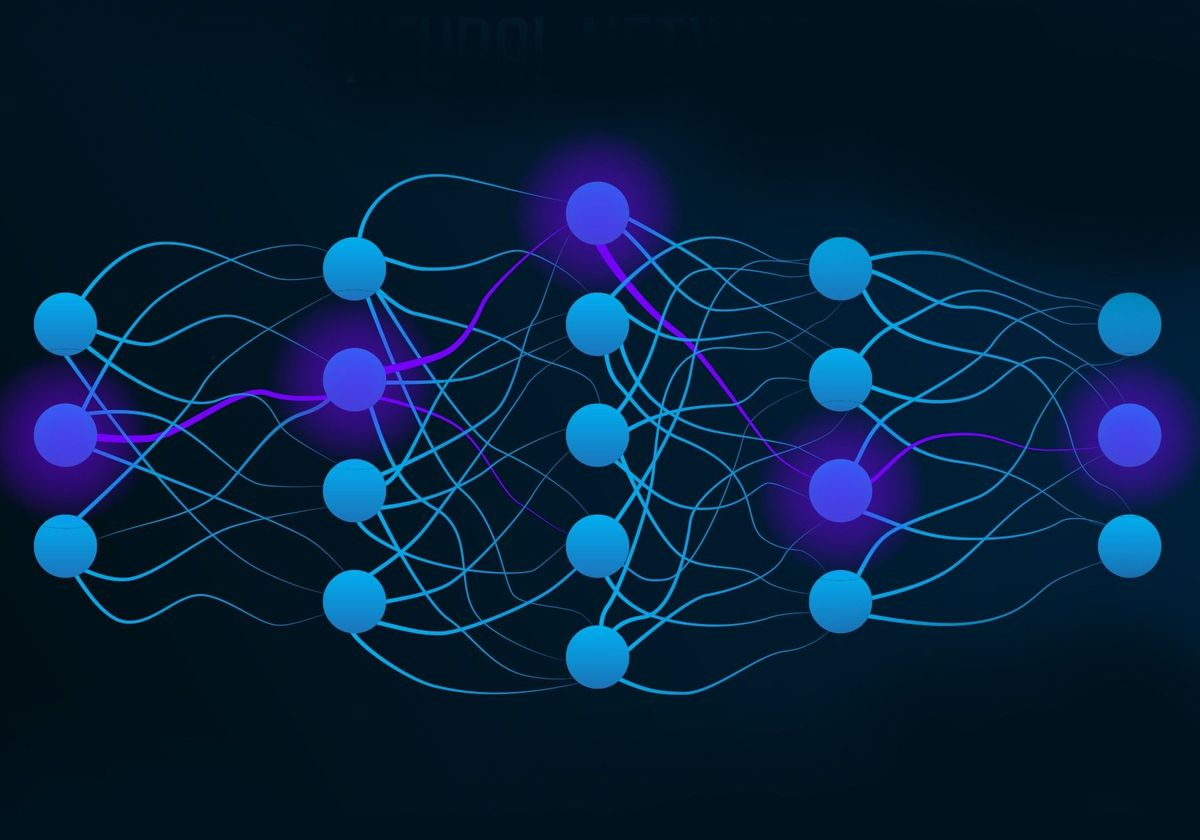
\includegraphics[scale=0.1]{figures/neurnet.jpg}  
\end{figure}

\end{itemize}
\end{frame}

\begin{frame}[allowframebreaks]{Experimental observations}
\begin{itemize}
    \item As an example in the image domain consider  the availability of a rendering engine that takes as an input a computer program describing a scene (coordinates of objects, textures, light sources, auxiliary labels, etc ...). $V=\text{rendering}(X)$.\\
    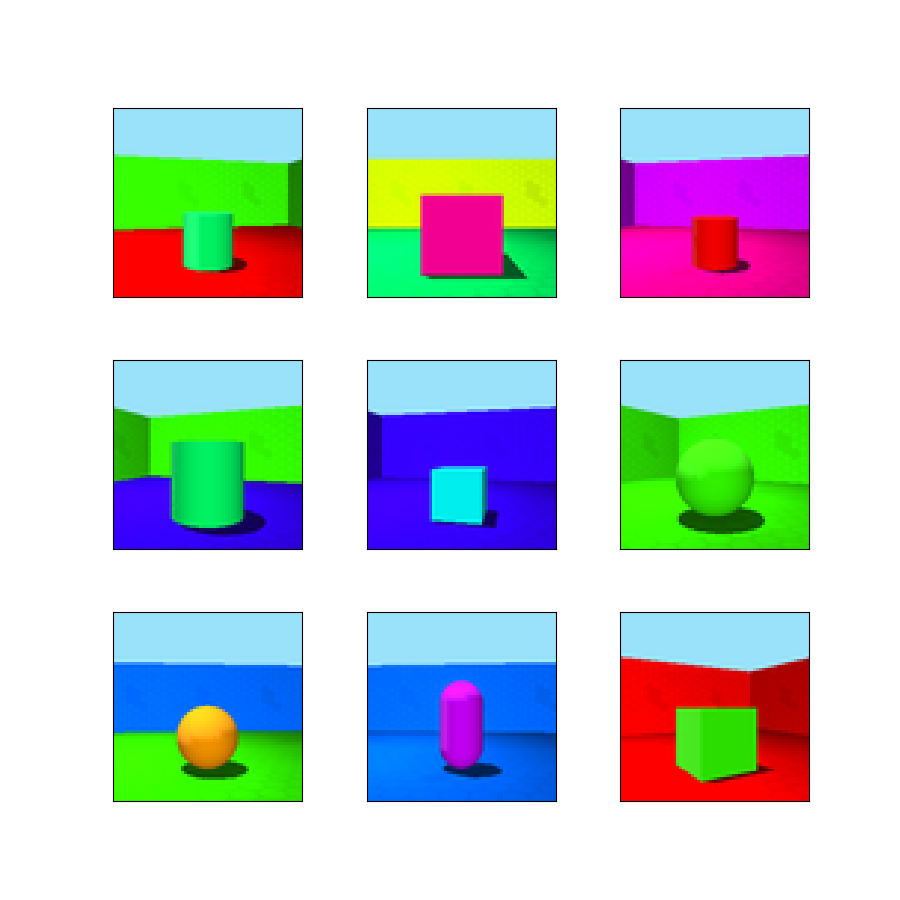
\includegraphics[scale=0.2]{figures/shapes3d-2.0.0.png}
\framebreak

\item Test of theory on generative diffusion models on the Shapes3D dataset (known ground truth latent factors of the rendering engine)
    \begin{figure}[htbp]
    \centering
    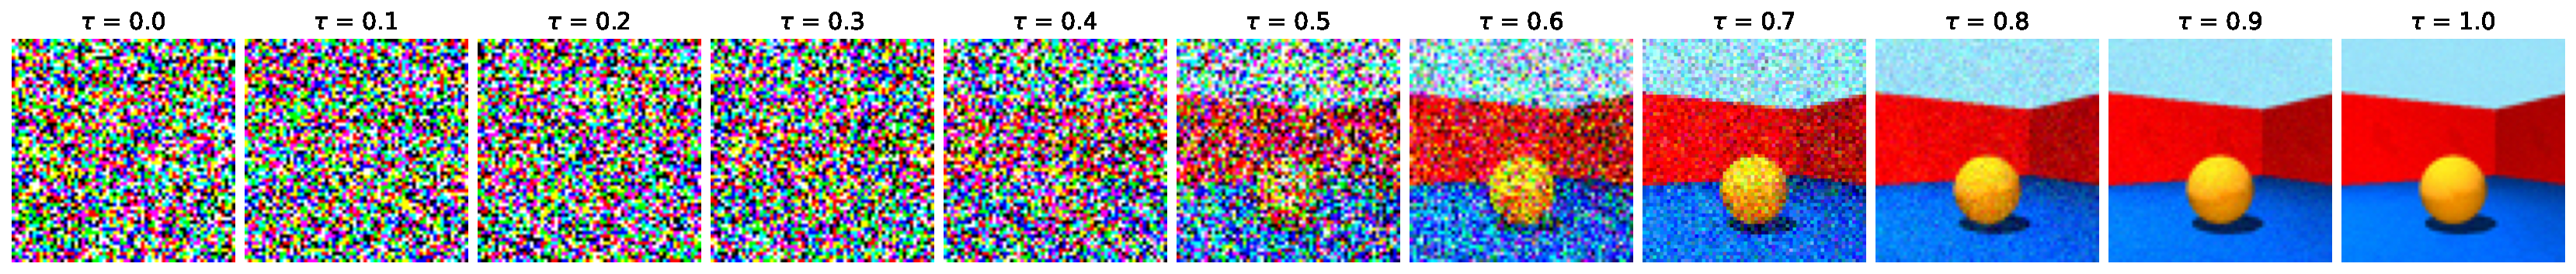
\includegraphics[width=\linewidth]{figures/noisy_balls.pdf}
    \caption{Evolution of generative dynamics vs $\tau$.}
    \label{fig:noise}
\end{figure}
\item These generative models can be understood under the lens of \textit{filtration} reduction: \begin{itemize}
    \item Dynamics which have access to $X$ are designed and simulated at training time
    \item We pretend to not having access to $X$ and construct a representation which does not depend on it
    \item We use such representation at test time to generate as many samples as we want
\end{itemize}
\framebreak
\item Simulation of the generative dynamics only have access to $Y_t$ and requires learning a drift $\langle\piphit,H\rangle$.
\item Will inspecting the internal activation of such drift allow to probe for the presence of latent factors?
\item Will it be consistent with the computation of Mutual Information?
\end{itemize}
\framebreak

Design of \textbf{forking} experiments:

\begin{figure}[htbp]
    \centering
    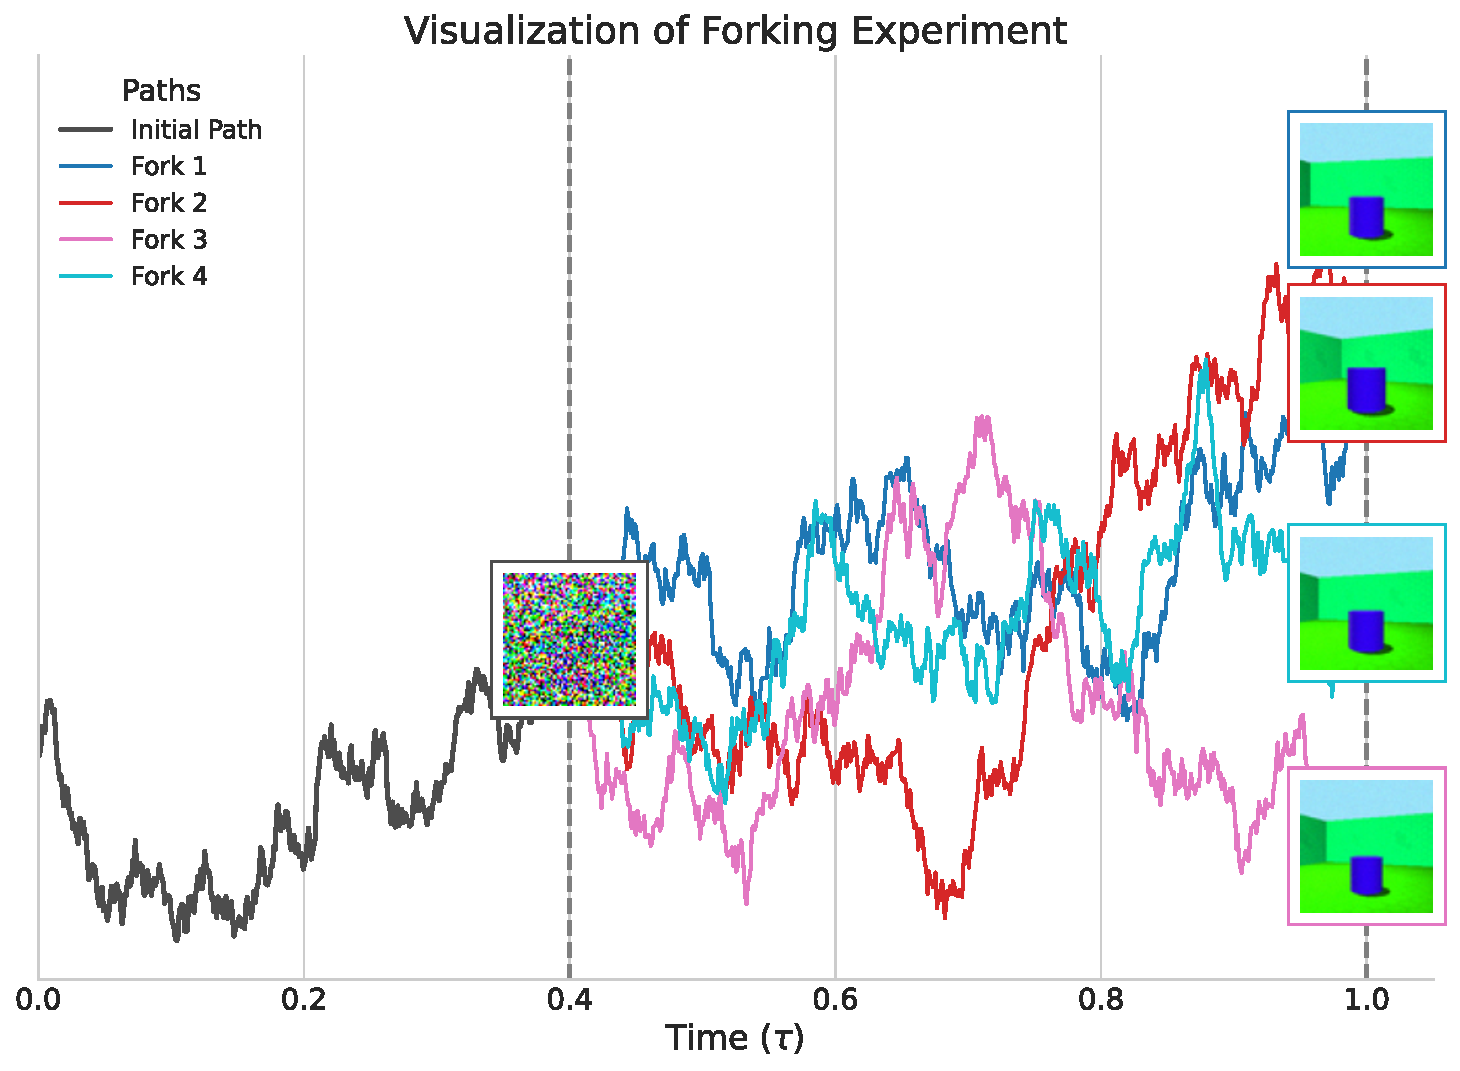
\includegraphics[width=0.6\linewidth]{figures/forking_visualization.pdf}
    \caption{  The image at time $\tau = 0.4$ is quite noisy. In the final generations after forking, the images exhibit coherence in the labels \textit{shape}, \textit{wall hue}, \textit{floor hue}, and \textit{object hue}. However, there is variation in \textit{orientation} and \textit{scale}.}
    \label{fig:forking_visualization}
\end{figure}
\framebreak

We probe linearly on the activations of the drift $\langle\piphit,H\rangle$:
\begin{figure}[htbp]
    \centering
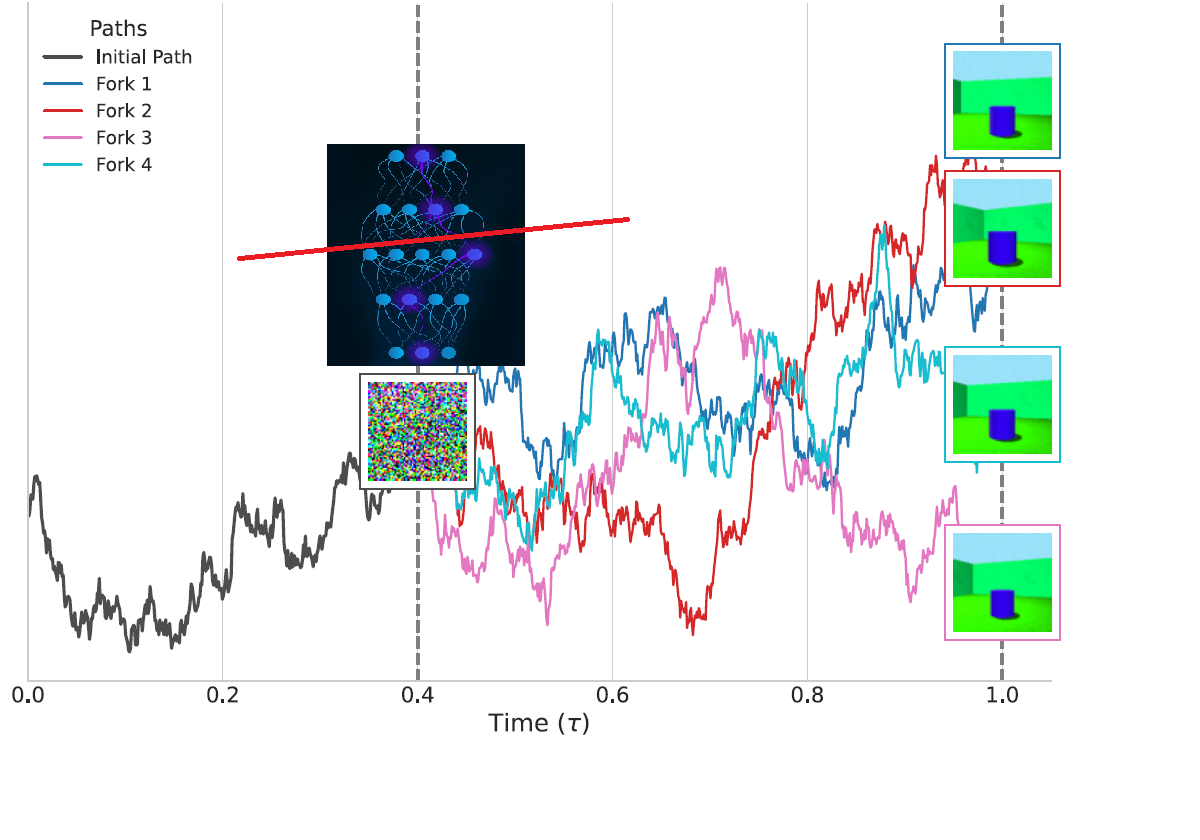
\includegraphics[scale=0.28]{figures/prob.png}
\end{figure}

\begin{figure}[htbp]
    \centering
    %\includegraphics[width=\linewidth]
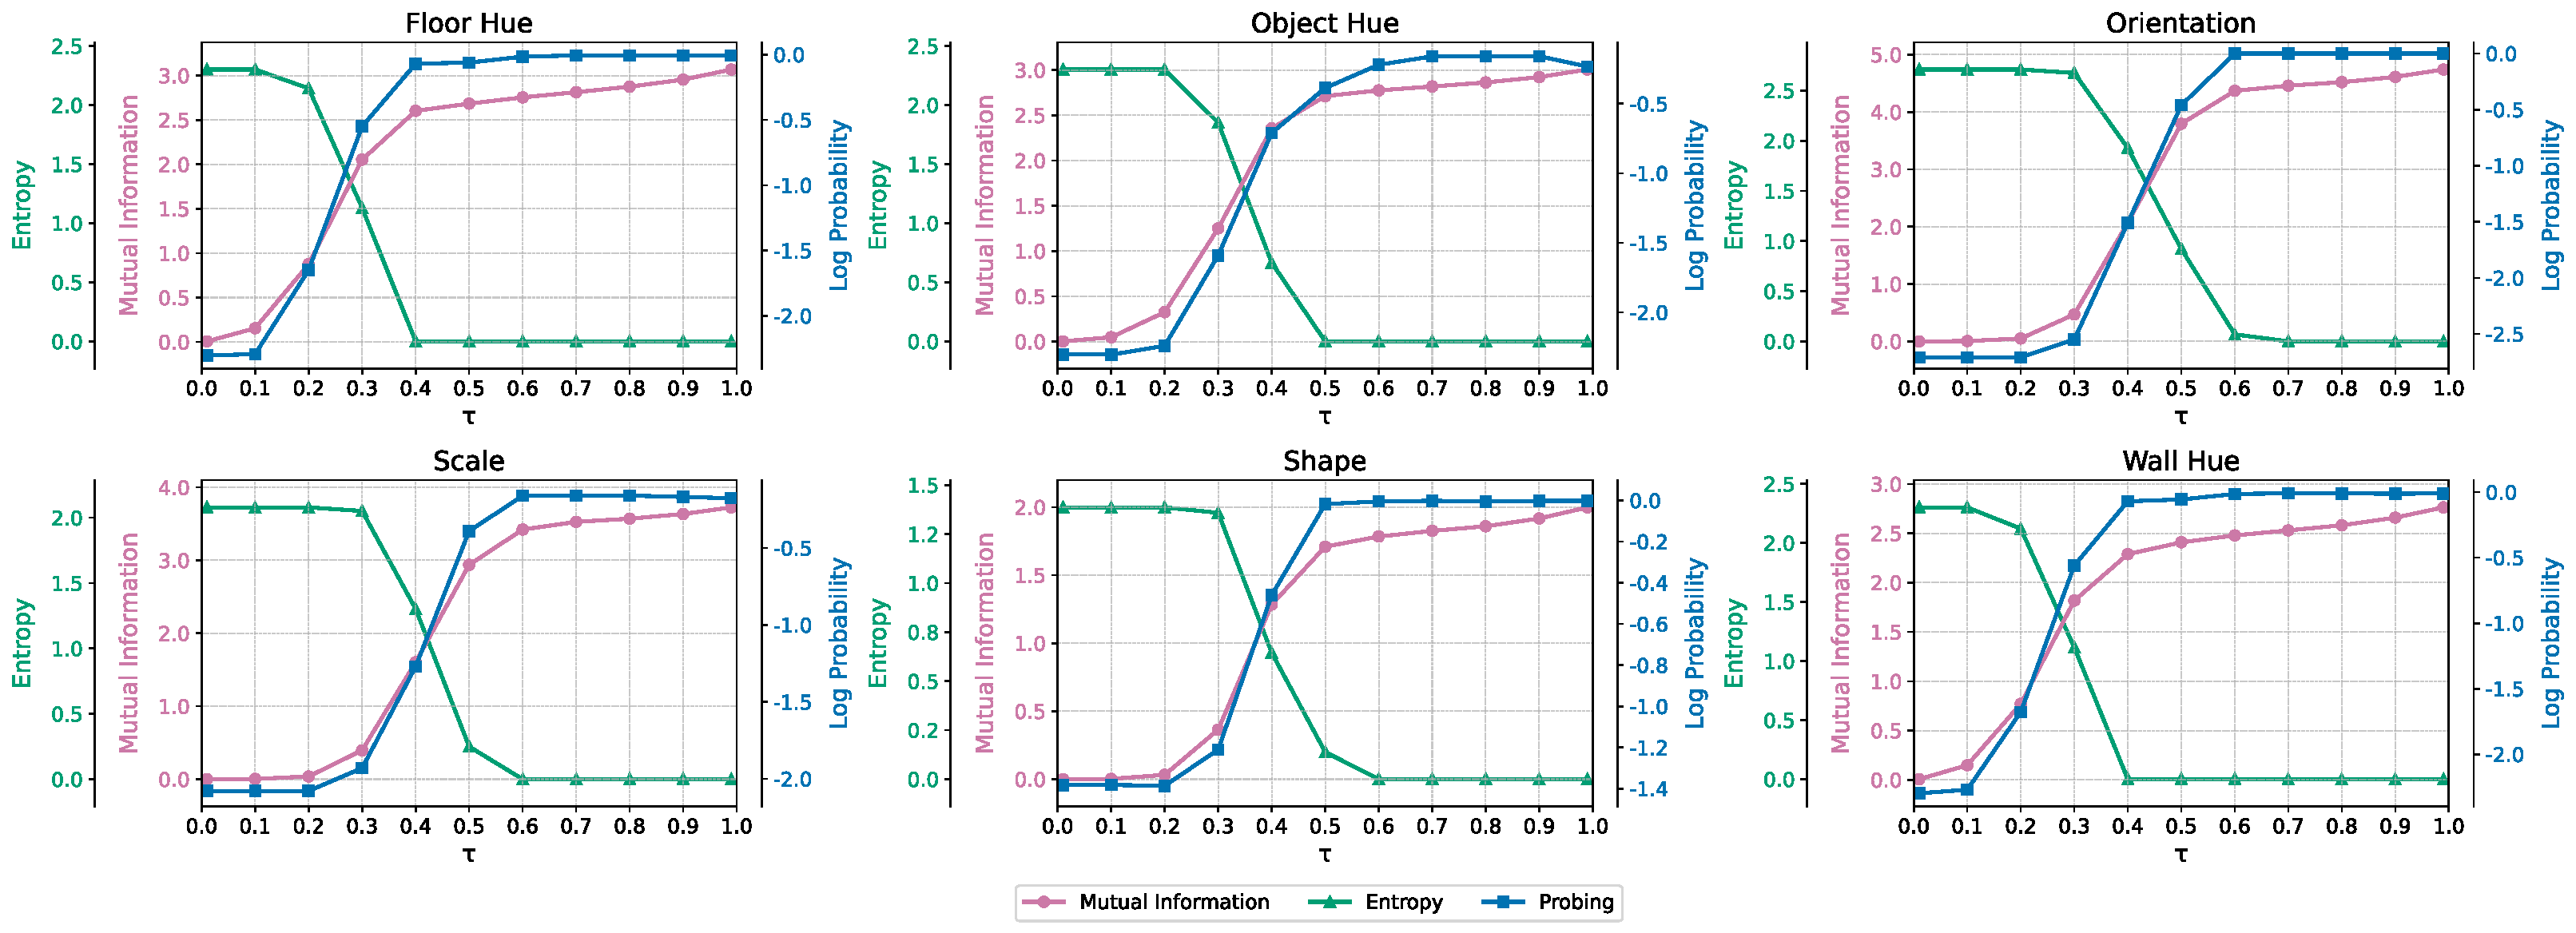
\includegraphics[scale=0.21]{figures/combined_plot.pdf}
    \caption{Mutual information, Entropy across forked generative pathways, and Probing results as functions of $\tau$.}
    \label{fig:forking_entropy_mi}
\end{figure}

\end{frame}

\begin{frame}{Some perspectives}
\begin{itemize}
    \item The mutual information computation can be used to understand the when and how of the emergence of the latent abstractions
    \item The nonlinear filtering perspective allows in principle to construct many more generative models
    \item We are currently investigating from a mechanistic interpretability perspective how \textit{Zakai equations} are implemented in generic classes of generative models
    \item Very strong signal for HMM (discrete time, discrete state-space)
    \item All the theory extends to time-varying $X_t$ (provided technical conditions...)
\end{itemize}
    
\end{frame}


\begin{frame}{}%[standout]
\centering	
\Huge{Thank you!! \\ Questions?}

\end{frame}

\begin{frame}{References}

\begin{thebibliography}{9}


\bibitem{latent}
Franzese et al, Latent Abstractions in Generative Diffusion Models, Entropy, MDPI 2025



\end{thebibliography}





    
\end{frame}


\begin{frame}{Linear H: special case}
\begin{itemize}
    \item Select the function $H$ as
   \begin{equation}
       H(Y_t,X,t)=\frac{1}{2}Y_t -\frac{\exp(-\frac{(T-t)}{2})V-Y_t}{1-\exp(-(T-t))}
   \end{equation}
\item $\E[H(Y_t,X,t) \g \cF^Y_t]=\frac{1}{2}Y_t -\frac{\exp(-\frac{(T-t)}{2})\E[V \g \sigma(Y_t)]-Y_t}{1-\exp(-(T-t))}$
\item The generative dynamics have then form $\dd Y_t=\frac{1}{2}Y_t -\frac{\exp(-\frac{(T-t)}{2})\E[V \g \sigma(Y_t)]-Y_t}{1-\exp(-(T-t))}+\dd W^{\cF^Y}_t$ (cfr with beginning of presentation!)
\item Those dynamics can be interpreted as \textbf{implicit} simulation of the system eq.\ref{eq:system}
    \end{itemize}
\end{frame}

\begin{frame}[allowframebreaks]{Enlargment of Filtrations}

	
    \begin{itemize}
    \item Consider the \textit{{reversed}} process $\hat{Y}_t\defeq Y_{T-t}$ defined on $\ccU$ and the corresponding filtration $\cF_t^{\hat{Y}}\defeq\sigma(\hat{Y}_{0\leq s\leq t})$. 
    \item The measure $\PO$ is selected such that the process $\hat{Y}_t$ has a $\cF_t^{\hat{Y}}$-adapted expression
	\begin{equation}\label{eq:diffmod_gen}
		\hat{Y}_t=\rX+\int\limits_{0}^t F(\hat{Y}_{s},s)\dd s+\hat{W}_t,%=\exp(-\alpha t)\hat{Y}_0+\hat{W}_t,
		%\rightarrow Y_{T-t}=Y_T+\alpha \int\limits_{T-t}^{T} Y_{s}\dd s+\hat{W}_t
	\end{equation}
	where $\{\hat{W}_t,\cF_t^{\hat{Y}}\}$ is a Brownian motion. 
    \item Then, Assumption 1 is valid since $Y_T=\hat{Y}_0=\rX$. 
    \item Using simple algebra, it holds that 
	$$Y_{t}=Y_0-\int\limits_{0}^{t} F(Y_{s},T-s)\dd s+\left(-Y_0+ \rX+\int\limits_{0}^{T} F(Y_{s},T-s)\dd s+\hat{W}_{T-t}\right),$$ 
	where the last term in the parentheses is equal to $-\hat{W}_T+\hat{W}_{T-t}$. 
	
\item 	Note that $\cF_t^{Y}=\sigma(\hat{Y}_{T-t\leq s\leq T})$. % is a \textit{decreasing} filtration.
	% , from the perspective of the reverse process. 
	Since $\sigma(\hat{Y}_{T-t\leq s\leq T})=\sigma(\hat{W}_{T-t\leq s\leq T})\cup \sigma(\hat{Y}_{T-t})$, $-\hat{W}_T+\hat{W}_{T-t}-\int_0^t\nabla\log \hat{p}(Y_s,T-s)\dd s$ is a Brownian motion adapted to $\cF^Y_t$, where this time $\PO(\hat{Y}_t\in \dd y)=\hat{p}(y,t)\dd y$. 
  \end{itemize}  
  \framebreak
  \begin{Theorem}\label{anders_thm}
		Consider the stochastic process $Y_t$ which solves Eq. \ref{eq:diffmod_gen}. The same stochastic process also admits a $\cF^Y_t$-adapted representation
		\begin{equation}\label{eq:songsde_gen}
			Y_t=Y_0+\int_0^t \underbrace{-F(Y_s,T-s)+\nabla\log \hat{p}(Y_s,T-s)}_{ F'(Y_s,s)}\dd s  +W_t.
		\end{equation}
	\end{Theorem}
Proof [Pardoux 2006].

We showed that a $\cF^Y$-adapted filtration can be linked to the reverse, $\cF^{\hat{Y}}$-adapted process induced by a forward diffusion \gls{SDE}.
 \framebreak
 \begin{itemize}
     \item From before, it is clear how to go from an $\cF^{Y,X}$-adapted filtration to a $\cF^Y$-adapted one
     \item What remains to be discussed is the connection that exists between the $\cF^Y$-adapted filtration, and its \textit{{enlarged}} version $\cF^{Y,X}$.
 \end{itemize}
\framebreak

\begin{Theorem}\label{theo:connection}
		Suppose that on $\ccU$, the Markov stochastic process $Y_t$ satisfying
		\begin{equation*}\label{gendir}
			Y_t=Y_0+\int_0^t F'(Y_s,s)\dd s+W_t,
		\end{equation*}
		where $\{W_{0\leq t\leq T},\cF^Y_{0\leq t\leq T}\}$ is a Brownian motion.
        Moreover, let Assumption 1 hold. Then, the same process admits $\ctF_t=\sigma(Y_{0\leq s\leq t},Y_T)$-adapted representation
		\begin{equation}\label{bridge}
			Y_t=Y_0+\int_0^t F'(Y_s,s)+\nabla_{Y_s}\log p(Y_T\g Y_s)\dd s+\beta_t,
		\end{equation}
		where $p(Y_T\g Y_s)$ is the density with reference to the Lebesgue measure of the probability $\PO(Y_T\g \sigma(Y_s))$, and $\{\beta_{0\leq t\leq T},\ctF_{0\leq t\leq T}\}$ is a Brownian motion.
	\end{Theorem}
    
\framebreak

    
Interestingly, in [Al-Hussaini et al.,  1987] it is proved that $\beta_t$ is a Brownian Motion using time-reversal techniques! 

Since $\hat{p}(y,T-t)={p}(y,t)$, the enlarged filtration version of \ref{eq:songsde_gen} reads 
	\begin{equation}\label{anders_them_2}
		Y_t=Y_0+\int_0^t \underbrace{-F(Y_s,T-s)+\nabla_{Y_s}\log p(Y_s\g Y_T)\dd s}_{\text{Equivalent to }H(Y_t,X,t)=-F(Y_s,T-s)+\nabla_{Y_s}\log p(Y_s\g \rX)}  +W_t.
	\end{equation}
	
\end{frame}

